\documentclass[a4paper,11pt]{article}
\usepackage{polski}
\usepackage[utf8]{inputenc}

% \usepackage{a4wide}

\usepackage{amsmath}
\usepackage{amsfonts}
% \usepackage{amssymb}
% \usepackage{amsthm}
\usepackage{listings}
\usepackage{graphicx}



\title{
  \textbf{Pracownia 35}\\
  {\Large Podstawy elektroniki, elektrotechniki i miernictwa}
}
\author{Rafał Łasocha}
\setcounter{equation}{0}

\begin{document}

\maketitle

\section{Zagadnienia teoretyczne}

\subsection{Szyna IEC-625}
Jest to magistrala służąca do komunikacji urządzeń laboratoryjnych z komputerem, opracowana przez HP w latach 70. Każde z urządzeń ustawia \textbf{numer selekcyjny urządzenia}, robi się to przez ustawienie pięciu przełączników binarnych np. z tyłu urządzenia. Przewody mogą mieć długość do 20m. Jest to złącze 24 pinowe.

\subsection{Dioda LED}
Jest to dioda, która jest zaliczana do przyrządów optoelektronicznych. Emituje promieniowanie w zakresie światła widzialnego, podczerwieni i ultrafioletu.

\subsection{Dioda prostownicza}
Dioda służąca do prostowania prądu przemiennego, charakteryzuje się możliwością przewodzenia prądu o dużym natężeniu.

\subsection{Dioda Zenera}
Dioda półprzewodnikowa. Przy polaryzacji zaporowej, po przekroczeniu pewnego napięcia, zaczyna gwałtownie przewodzić prąd.


\section{Przebieg ćwiczenia}

Na początku wzięliśmy pierwszy z układów i podłączyliśmy go do multimetrów i zasilacza tak jak zostało to przedstawione w zadaniu. Następnie sprawdziliśmy jakie adresy mają przypisane poszczególne urządzenia i wpisaliśmy te informacje w konfiguracji programu \texttt{Pomiary\_IU}, służącemu do pomiarów charakterystyk prądowo napięciowych. Ustawiliśmy również timeout na 1 sekundę oraz ograniczenie prądowe na 300mAh.

W każdej próbie najpierw ustawialiśmy większy zakres napięć zasilania oraz większy krok napięcia (0.5 - 1V), a następnie po zobaczeniu jak w przybliżeniu przedstawia się wykres, zawężaliśmy zakres napięć i znacznie zmniejszaliśmy krok.

\subsection{Dioda LED}

Pierwszym podłączonym układem był ten z diodą LED. Został użyty opornik 990 Ohm. Charakterystyka prądowo - napięciowo przedstawiona jest na rysunku 1.

\begin{figure}[ht]
 \begin{center}
  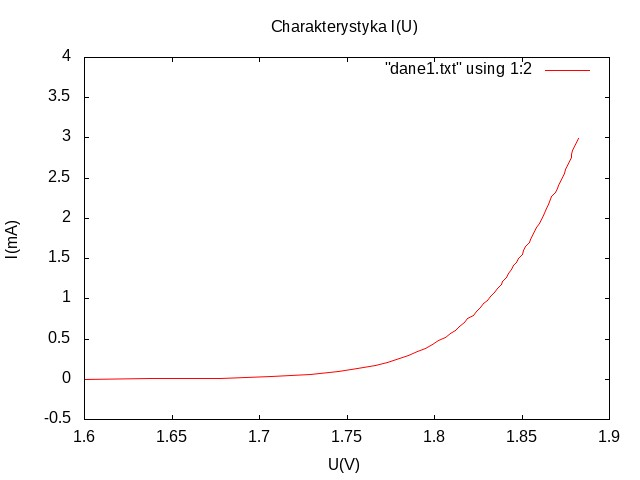
\includegraphics[width=12cm]{wykres1}
 \end{center}
 \caption{Dioda LED}
\end{figure}

\subsection{Dioda prostownicza}

Drugim podłączonym układem był ten z diodą prostowniczą. Został użyty opornik 2kOhm. Charakterystyka prądowo - napięciowo przedstawiona jest na rysunku 2.

\begin{figure}[ht]
 \begin{center}
  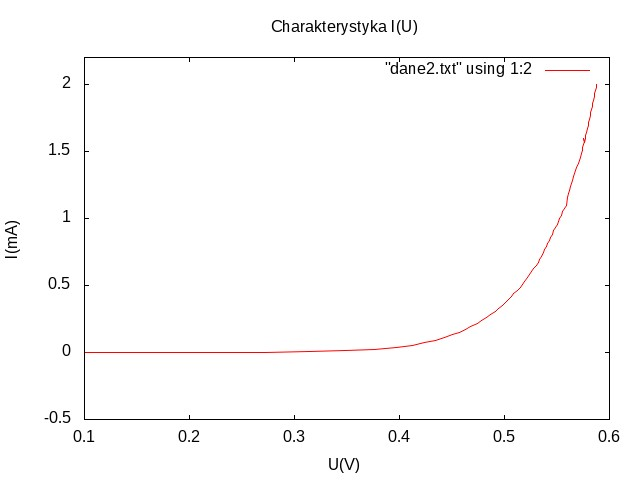
\includegraphics[width=12cm]{wykres2}
 \end{center}
 \caption{Dioda prostownicza}
\end{figure}

\subsection{Dioda Zenera}

Ostatnią podłączoną diodą była dioda Zenera. Został użyty opornik 2kOhm. Charakterystyka prądowo - napięciowo przedstawiona jest na rysunku 3.

\begin{figure}[ht]
 \begin{center}
  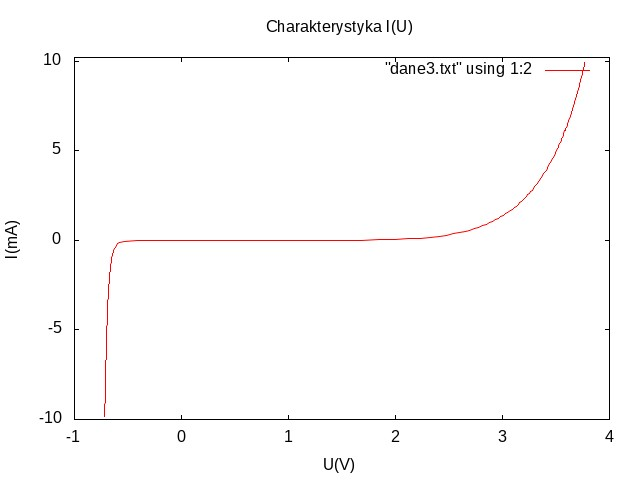
\includegraphics[width=12cm]{wykres3}
 \end{center}
 \caption{Dioda Zenera}
\end{figure}


\section{Wnioski}

Dzięki tej pracowni dowiedzieliśmy się co można realizować przy użyciu urządzeń połączonych magistralą IEC-625. Można napisać programy korzystające z tej magistrali, aby znacznie uprościć  i zautomatyzować pobieranie pomiarów. Ponadto tak pobrane pomiary nie są obarczone błędem ludzkim. Oczywiście dowiedzialiśmy się też jak wyglądają charakterystyki poszczególnych diód, szczególnie ciekawym wykresem jest charakterystyka prądowo-napięciowa diody Zenera.



\end{document}